\documentclass[conference]{IEEEtran}
\IEEEoverridecommandlockouts

\usepackage[utf8]{inputenc}
\usepackage[T1]{fontenc}
\usepackage[brazil]{babel}
\usepackage{cite}
\usepackage{amsmath,amssymb,amsfonts}
\usepackage{graphicx}
\usepackage{textcomp}
\usepackage{xcolor}
\usepackage{url}
\usepackage{booktabs}
\usepackage{array}
\usepackage{listings}
\usepackage{balance}

\definecolor{codebg}{RGB}{248,248,248}
\definecolor{codekw}{RGB}{0,73,122}
\definecolor{codecm}{RGB}{82,110,72}
\definecolor{codestr}{RGB}{150,60,40}

\lstdefinestyle{homescript}{
  backgroundcolor=\color{codebg},
  basicstyle=\ttfamily\scriptsize,
  keywordstyle=\color{codekw}\bfseries,
  commentstyle=\color{codecm}\itshape,
  numbers=left, numberstyle=\tiny\color{gray}, numbersep=5pt,
  frame=single, breaklines=true, columns=fullflexible,
  keepspaces=true, showstringspaces=false, tabsize=2,
  morekeywords={device,sensor,pin,type,trig,echo,turn,on,off,wait,
    if,else,for,while,when,detected,not_detected,let,print,
    dispositivo,pino,tipo,gatilho,eco,ligar,desligar,esperar,
    se,senao,para,enquanto,quando,detectado,nao_detectado}
}

\lstdefinestyle{csmall}{
  backgroundcolor=\color{codebg}, language=C,
  basicstyle=\ttfamily\scriptsize,
  keywordstyle=\color{codekw}\bfseries,
  commentstyle=\color{codecm}\itshape,
  numbers=left, numberstyle=\tiny\color{gray}, numbersep=5pt,
  frame=single, breaklines=true, columns=fullflexible,
  keepspaces=true, showstringspaces=false, tabsize=2
}

\def\BibTeX{{\rm B\kern-.05em{\sc i\kern-.025em b}\kern-.08em
    T\kern-.1667em\lower.7ex\hbox{E}\kern-.125emX}}

\begin{document}

\title{HomeScript: Projeto e Implementação de uma Linguagem de\\
Domínio Específico e Compilador para Automação Residencial com Arduino}

\author{
\IEEEauthorblockN{Enzo Perroni}
\IEEEauthorblockA{Ciência da Computação\\IBMEC Rio de Janeiro\\Rio de Janeiro, Brasil}
\and
\IEEEauthorblockN{João Pedro Giovanelli}
\IEEEauthorblockA{Ciência da Computação\\IBMEC Rio de Janeiro\\Rio de Janeiro, Brasil}
\and
\IEEEauthorblockN{Arthur Schiller}
\IEEEauthorblockA{Ciência da Computação\\IBMEC Rio de Janeiro\\Rio de Janeiro, Brasil}
\and
\IEEEauthorblockN{Arthur Camaz}
\IEEEauthorblockA{Ciência da Computação\\IBMEC Rio de Janeiro\\Rio de Janeiro, Brasil}
\and
\IEEEauthorblockN{Maria Claudia}
\IEEEauthorblockA{Ciência da Computação\\IBMEC Rio de Janeiro\\Rio de Janeiro, Brasil}
}

\maketitle

% -------------------------------------------------------
\begin{abstract}
Programar automações residenciais em Arduino exige conhecimento de C/C++,
configuração explícita de pinos, seleção entre \texttt{digitalRead} e
\texttt{analogRead}, inicialização de bibliotecas de sensores e estruturação
manual das funções \texttt{setup()} e \texttt{loop()}. Esse nível de detalhe
constitui uma barreira significativa para usuários que compreendem a regra de
automação desejada, mas não dominam programação embarcada. Este artigo
apresenta o \textbf{HomeScript}, uma linguagem de domínio específico (DSL)
bilíngue — inglês e português — e um compilador completo que transforma
arquivos \texttt{.iot} em código C/Arduino funcional. O compilador implementa
as quatro fases canônicas: análise léxica com 40 classes de tokens, análise
sintática por parser recursivo descendente com construção de Árvore Sintática
Abstrata (AST), análise semântica com tabela de símbolos e controle de escopo,
e geração de código com suporte nativo a sensores DHT11 e HC-SR04. O sistema
inclui uma interface de linha de comando com saída JSON estruturada, um backend
REST em FastAPI e uma IDE web em React com Monaco Editor, rastreio passo a
passo do pipeline de compilação e construtor visual de automações. A validação
foi realizada sobre hardware físico (Arduino Uno, ATMega328P) utilizando o
cenário residencial completo — \texttt{casa\_completa\_plus.iot} — com 9
atuadores e 6 sensores. O código C gerado automaticamente pelo compilador foi
embarcado sem alteração manual e operou corretamente, confirmando a corretude
do pipeline de compilação de ponta a ponta.
\end{abstract}

\begin{IEEEkeywords}
compilador, linguagem de domínio específico, automação residencial, sistemas
embarcados, geração de código
\end{IEEEkeywords}

% -------------------------------------------------------
\section{Introdução}
\label{sec:intro}

A proliferação de dispositivos conectados impulsiona a automação residencial
como um dos segmentos de maior crescimento da Internet das Coisas
(IoT)~\cite{atzori2010,alfuqaha2015}. Estima-se que dezenas de bilhões de
dispositivos IoT estarão em operação antes do fim desta
década~\cite{zanella2014}, com aplicações que vão desde o simples controle de
luminosidade até sistemas integrados de segurança, climatização e irrigação.

A plataforma Arduino~\cite{banzi2011} consolidou-se como padrão de
prototipagem nesse domínio por seu ecossistema de bibliotecas e baixo custo.
Entretanto, mesmo tarefas elementares exigem código não trivial. Ligar uma
lâmpada ao detectar movimento requer: declarar um pino como \texttt{OUTPUT}
com \texttt{pinMode}, configurar o pino do sensor como \texttt{INPUT},
chamar \texttt{digitalRead} dentro do \texttt{loop()}, comparar o resultado
com \texttt{HIGH} e invocar \texttt{digitalWrite}. Para sensores
especializados — como o DHT11 (temperatura/umidade) ou o HC-SR04
(ultrassom) — somam-se a inclusão de bibliotecas externas, inicialização de
objetos, tratamento de leituras inválidas e protocolos de temporização de
pulso (\texttt{pulseIn}). Esse nível de detalhe cria uma barreira real para
usuários que entendem \emph{o quê} querem automatizar, mas não
\emph{como} o hardware funciona.

Linguagens de domínio específico (DSLs) são uma solução consolidada para
exatamente esse tipo de problema~\cite{mernik2005,fowler2010,vandeursen2000}.
Ao contrário de linguagens de propósito geral, uma DSL restringe o espaço de
expressão ao conjunto de conceitos relevantes para um domínio, tornando
programas menores, mais legíveis e menos suscetíveis a erros de baixo nível.
SQL, HTML e VHDL são exemplos canônicos. A teoria de compiladores, formalizada
por Aho et al.~\cite{aho2006} e Cooper \& Torczon~\cite{cooper2011}, fornece
o arcabouço para transformar uma DSL em código executável por meio de fases
bem definidas de análise e síntese.

O projeto \textbf{HomeScript} foi concebido nesse contexto com dois objetivos
complementares. O objetivo \emph{acadêmico} é implementar, a partir dos
fundamentos teóricos, um compilador completo com todas as fases canônicas,
sem ferramentas de geração automática como Lex/Yacc ou
ANTLR~\cite{parr2013}. O objetivo \emph{prático} é criar uma ferramenta
genuinamente utilizável, com interface web, construtor visual e suporte
bilíngue (inglês e português), que gere código Arduino correto a partir de
uma descrição declarativa de regras de automação.

A listagem~\ref{lst:intro} ilustra uma automação básica em HomeScript. O
compilador transforma esse arquivo em código C com \texttt{setup()},
\texttt{loop()}, \texttt{pinMode} e \texttt{digitalRead} — sem que o
usuário precise conhecer esses detalhes.

\begin{lstlisting}[style=homescript,caption={Automação básica em HomeScript.},label={lst:intro}]
device luz pin 13;
sensor movimento pin 2;

when movimento == detected {
    turn luz on;
    wait 5000;
    turn luz off;
}
\end{lstlisting}

O restante deste artigo está organizado da seguinte forma. A
Seção~\ref{sec:linguagem} define a linguagem HomeScript. A
Seção~\ref{sec:compilador} detalha a implementação das quatro fases do
compilador. A Seção~\ref{sec:sistema} apresenta o sistema integrado, a IDE
web, o cenário de validação, o código C gerado e os resultados com hardware
físico. A Seção~\ref{sec:conclusao} conclui e aponta trabalhos futuros.

% -------------------------------------------------------
\section{HomeScript: Definição e Design da Linguagem}
\label{sec:linguagem}

\subsection{Princípios de Design}

A definição da linguagem seguiu três princípios fundamentais, derivados dos
critérios de Mernik et al.~\cite{mernik2005} para desenvolvimento de DSLs:

\begin{enumerate}
\item \textbf{Proximidade com a linguagem natural.} Comandos como
\texttt{turn luz on} e \texttt{wait 1000} devem ser compreensíveis sem
documentação.
\item \textbf{Correspondência direta com operações de hardware.} Cada
construção mapeia para chamadas Arduino bem definidas, sem ambiguidade.
\item \textbf{Bilinguismo nativo.} Palavras-chave em português são sinônimos
no nível léxico, sem impacto no parser ou gerador.
\end{enumerate}

\subsection{Declarações de Hardware}

\subsubsection{Dispositivos}
Representam atuadores digitais. A declaração \texttt{device nome pin N;}
gera \texttt{\#define nome N} e \texttt{pinMode(nome, OUTPUT)}.
A forma PT-BR usa \texttt{dispositivo}/\texttt{pino}.

\subsubsection{Sensores}
Há quatro categorias com comportamento distinto:
\begin{itemize}
\item \textbf{Digital genérico} (\texttt{pin N}): lido com
\texttt{digitalRead}. Comparações usam \texttt{detected}/\texttt{not\_detected}.
\item \textbf{Analógico} (\texttt{pin AN}): lido com \texttt{analogRead}.
Comparações obrigatoriamente numéricas.
\item \textbf{DHT11} (\texttt{type dht11 pin N}): objeto \texttt{DHT},
\texttt{readTemperature()} com guarda \texttt{!isnan()}.
\item \textbf{HC-SR04} (\texttt{type hcsr04 trig N echo N}): função auxiliar
com \texttt{pulseIn}.
\end{itemize}

\subsection{Variáveis e Expressões}

Variáveis inteiras são declaradas com \texttt{let nome = expr;}. Expressões
suportam \texttt{+}, \texttt{-}, \texttt{*}, \texttt{/} com precedência
convencional e agrupamento por parênteses.

\subsection{Estruturas de Controle}
\label{subsec:controle}

\texttt{if}/\texttt{se} e \texttt{when}/\texttt{quando} aceitam condição,
bloco obrigatório e \texttt{else}/\texttt{senao} opcional. Laços
\texttt{while}/\texttt{enquanto} e \texttt{for}/\texttt{para} suportam
tanto variáveis quanto sensores como condição, com leitura reavaliada
a cada iteração.

\subsection{Sistema de Tokens}

O lexer reconhece 40 classes de tokens. A Tabela~\ref{tab:tokens} apresenta
as categorias principais.

\begin{table}[htbp]
\caption{Classes de tokens da linguagem HomeScript}
\label{tab:tokens}
\centering
\begin{tabular}{p{0.21\linewidth}p{0.20\linewidth}p{0.47\linewidth}}
\toprule
\textbf{Categoria} & \textbf{Exemplos} & \textbf{Padrão} \\
\midrule
Palavra-chave EN & \texttt{device}, \texttt{when} & Verificação pós-identificador \\
Palavra-chave PT & \texttt{dispositivo}, \texttt{quando} & Mesmo mecanismo \\
Identificador & \texttt{luz}, \texttt{temp1} & \texttt{[a-zA-Z\_][a-zA-Z0-9\_]*} \\
Número & \texttt{13}, \texttt{1000} & \texttt{[0-9]+} \\
Pino analógico & \texttt{A0}, \texttt{A1} & \texttt{A[0-9]+} (prioridade) \\
Op. relacional & \texttt{==}, \texttt{!=}, \texttt{>=} & Lookahead de 1 char \\
Op. aritmético & \texttt{+}, \texttt{-}, \texttt{*}, \texttt{/} & Char único \\
Delimitadores & \texttt{\{}, \texttt{\}}, \texttt{;} & Char único \\
Especiais & \texttt{EOF}, erro & Fim de arquivo / char inválido \\
\bottomrule
\end{tabular}
\end{table}

% -------------------------------------------------------
\section{Implementação do Compilador}
\label{sec:compilador}

\subsection{Visão Geral da Arquitetura em Fases}

O compilador foi implementado integralmente em C (C99), sem dependências
externas, em quatro módulos independentes: \texttt{lexer/},
\texttt{parser/} (com AST), \texttt{semantic/} e \texttt{codegen/}.
O executável \texttt{compiler/main.c} integra as fases. A decisão de não
usar geradores automáticos~\cite{parr2013} foi intencional: implementar
cada fase manualmente expõe o funcionamento interno do pipeline, atendendo
ao objetivo pedagógico do projeto~\cite{aho2006,cooper2011}.

\subsection{Análise Léxica}

O lexer mantém estado com quatro campos: \texttt{FILE *arquivo},
\texttt{char caractere\_atual}, \texttt{int linha} e \texttt{int coluna}.
A função \texttt{lexer\_proximo\_token()} executa:

\textbf{1.} Pular espaços e comentários de linha (\texttt{//}) via
\texttt{lexer\_pular\_insignificantes()}.

\textbf{2.} Verificar o caractere atual e despachar:
\begin{itemize}
\item \texttt{c == 'A'} e próximo é dígito $\Rightarrow$ pino analógico
(prioridade sobre identificadores).
\item \texttt{isalpha(c) || c=='\_'} $\Rightarrow$ identificador/palavra-chave.
A função \texttt{verificar\_palavra\_reservada()} compara contra 34
palavras-chave (17 EN + 17 PT-BR).
\item \texttt{isdigit(c)} $\Rightarrow$ número inteiro.
\item \texttt{c $\in$ \{'=','!','>','<'\}} $\Rightarrow$ operador com
lookahead de 1 caractere (via \texttt{fgetc}/\texttt{ungetc}) para
compostos: \texttt{==}, \texttt{!=}, \texttt{>=}, \texttt{<=}.
\item Operadores aritméticos e delimitadores: tokens de 1 caractere.
\item Qualquer outro: \texttt{TOKEN\_ERROR}.
\end{itemize}

\begin{lstlisting}[style=csmall,caption={Função principal do lexer.},label={lst:lexer}]
Token lexer_proximo_token(Lexer *lexer) {
    lexer_pular_insignificantes(lexer);
    if (lexer->eof)
        return criar_token(TOKEN_EOF, "EOF", ...);

    char c = lexer->caractere_atual;
    if (c=='A' && isdigit(lexer_espiar(lexer)))
        return lexer_ler_pino_analogico(lexer);
    if (isalpha(c) || c=='_')
        return lexer_ler_identificador(lexer);
    if (isdigit(c))
        return lexer_ler_numero(lexer);
    if (c=='='||c=='!'||c=='>'||c=='<')
        return lexer_ler_operador(lexer);
    /* operadores aritmeticos, delimitadores... */
}
\end{lstlisting}

Cada token carrega tipo, valor (\texttt{char[256]}), linha e coluna.
Essa informação de posição percorre todo o pipeline e é usada pelo frontend
para destacar erros no editor.

\subsection{Análise Sintática e AST}

\subsubsection{Estrutura da AST}
Definida em \texttt{parser/ast.h}, a AST usa representação uniforme: todos
os nós são \texttt{ASTNode}, com campos genéricos. Os 14 tipos de nó
(\texttt{NodeType}) incluem \texttt{NODE\_PROGRAM} (raiz),
\texttt{NODE\_DEVICE\_DECL}, \texttt{NODE\_SENSOR\_DECL},
\texttt{NODE\_VAR\_DECL}, \texttt{NODE\_ASSIGN\_CMD},
\texttt{NODE\_PRINT\_CMD}, \texttt{NODE\_TURN\_CMD},
\texttt{NODE\_WAIT\_CMD}, \texttt{NODE\_IF\_STMT},
\texttt{NODE\_WHEN\_STMT}, \texttt{NODE\_FOR\_STMT},
\texttt{NODE\_WHILE\_STMT}, \texttt{NODE\_BLOCK} e
\texttt{NODE\_CONDITION}.

Campos relevantes: \texttt{nome[64]}, \texttt{pino[64]},
\texttt{pino\_secundario[64]} (pino \texttt{echo} do HC-SR04),
\texttt{sensor\_tipo[64]}, \texttt{operador} (EQ, NE, GT, LT, GE, LE),
\texttt{valor\_comparacao[64]}, \texttt{estado} (ON/OFF),
\texttt{tempo\_espera} e \texttt{expressao[256]}. Cada nó suporta até 64
filhos e registra linha e coluna de origem.

\subsubsection{Parser Recursivo Descendente}
O parser~\cite{aho2006,wirth1976} é recursivo descendente (RDP), adequado
para gramáticas LL(1) onde cada produção é determinada pelo próximo token
sem backtracking. A função \texttt{parser\_analisar()} cria o nó raiz e
itera chamando \texttt{parser\_statement()} até EOF. Um dispatcher baseado
em \texttt{switch} seleciona a função de produção correta:

\begin{lstlisting}[style=csmall,caption={Dispatcher do parser.},label={lst:parser}]
static ASTNode* parser_statement(Parser *p) {
    switch (p->token_atual.tipo) {
      case TOKEN_DEVICE:    return parser_device_decl(p);
      case TOKEN_SENSOR:    return parser_sensor_decl(p);
      case TOKEN_LET:       return parser_var_decl(p);
      case TOKEN_TURN:
      case TOKEN_LIGAR:
      case TOKEN_DESLIGAR:  return parser_turn_cmd(p);
      case TOKEN_WAIT:      return parser_wait_cmd(p);
      case TOKEN_IF:        return parser_if_stmt(p);
      case TOKEN_FOR:       return parser_for_stmt(p);
      case TOKEN_WHILE:     return parser_while_stmt(p);
      case TOKEN_WHEN:      return parser_when_stmt(p);
      case TOKEN_IDENTIFIER: return parser_assign_cmd(p);
      default:
        parser_registrar_erro(p, "Comando nao reconhecido");
        return NULL;
    }
}
\end{lstlisting}

Expressões aritméticas usam hierarquia de três funções que codifica
precedência nas chamadas: \texttt{parser\_expressao()} (\texttt{+}/\texttt{-})
$\to$ \texttt{parser\_termo()} (\texttt{*}/\texttt{/}) $\to$
\texttt{parser\_fator()} (identificador, número, parênteses).

Um nó \texttt{for} possui sempre quatro filhos: \texttt{[init, cond, update, block]}. Nós condicionais possuem dois ou três: \texttt{[cond, then, [else]]}. O parser usa estratégia \textit{stop-on-first-error}: ao primeiro erro, produz mensagem com linha, coluna e token encontrado.

\subsection{Análise Semântica}

A análise semântica (\texttt{semantic/semantic.c}) verifica correção lógica.
A tabela de símbolos suporta até 256 entradas e 64 escopos aninhados.
Opera em dois passos: \texttt{coletar\_declaracoes\_fixas()} registra todos
os dispositivos e sensores globalmente; \texttt{analisar\_no()} valida cada
nó da AST. As verificações incluem:

\begin{itemize}
\item Identificadores duplicados no mesmo escopo.
\item Conflito de pinos entre dispositivos/sensores.
\item Trig e echo iguais no HC-SR04.
\item Dispositivo não declarado em \texttt{turn}/\texttt{ligar}.
\item Sensor inexistente em condição \texttt{if}/\texttt{when}.
\item DHT11 comparado com \texttt{detected} — erro de tipo semântico.
\item Atribuição para variável não declarada.
\item Identificador desconhecido em expressão aritmética.
\item Valor de condição que não é número, palavra reservada nem variável.
\end{itemize}

\subsection{Geração de Código C/Arduino}

O gerador (\texttt{codegen/codegen.c}) acumula código C em buffer estático
de 8 192 bytes. A geração é dividida em três partes: preâmbulo,
\texttt{setup()} e \texttt{loop()}.

\subsubsection{Preâmbulo}
Dispositivos geram macros \texttt{\#define nome pino}. Sensores genéricos
geram variáveis de pino (\texttt{int nome\_pin = N;}). Sensores DHT11
instanciam o objeto \texttt{DHT} e emitem \texttt{\#include <DHT.h>}. Sensores
HC-SR04 geram dois inteiros de pino e uma função auxiliar com \texttt{pulseIn}.

\subsubsection{Função \texttt{setup()}}
Dispositivos: \texttt{pinMode(nome, OUTPUT)}. Sensores genéricos:
\texttt{pinMode(pin, INPUT)}. DHT11: \texttt{sensor.begin()}. HC-SR04:
\texttt{OUTPUT}/\texttt{INPUT} para trig/echo e \texttt{LOW} inicial.
\texttt{Serial.begin(9600)} sempre emitido.

\subsubsection{Tradução de Condições e Cache de Leituras}
A tradução de condições depende do tipo de sensor. Para sensor digital com
\texttt{detected}: \texttt{digitalRead(pin) == HIGH}. Para analógico:
\texttt{analogRead(pin) op valor} com variável temporária. Para DHT11:
\texttt{!isnan(leit) \&\& leit op val}. Para HC-SR04: chamada à função
auxiliar.

O gerador implementa um \emph{cache de leituras}: quando um bloco
\texttt{if}/\texttt{else} e seu \texttt{else} imediato referenciam o mesmo
sensor, uma variável temporária é materializada antes do \texttt{if} e
reutilizada em ambos os ramos — fundamental para sensores lentos como DHT11
(que leva $\sim$250 ms por leitura). A detecção verifica se o primeiro filho
do bloco \texttt{else} é um \texttt{if}/\texttt{when} sobre o mesmo sensor.

Laços \texttt{while} e \texttt{for} são gerados com:
\begin{lstlisting}[style=csmall]
while (1) {
    if (!(condicao)) break;
    /* corpo */
}
\end{lstlisting}
Esse padrão reavalia a condição (e relê o sensor) a cada iteração sem
duplicar código.

\subsection{Interface de Linha de Comando e Saída JSON}

O executável \texttt{homescript} aceita: \texttt{--tokens}, \texttt{--ast},
\texttt{--code}, \texttt{--output F} e \texttt{--json}. O modo JSON
produz um objeto com campos \texttt{sucesso}, \texttt{erro}, \texttt{erros}
(array com fase, mensagem, linha, coluna), \texttt{tokens},
\texttt{ast} e \texttt{codigo\_c} — projetado para consumo pelo backend
Python sem parsing de saída textual.

% -------------------------------------------------------
\section{Sistema Integrado, Validação e Resultados}
\label{sec:sistema}

\subsection{Arquitetura do Sistema}

O sistema é composto por três camadas. O compilador C é autossuficiente como
ferramenta de linha de comando. O backend Python encapsula o compilador via
subprocesso. O frontend React consome a API REST. Essa separação garante
comportamento idêntico entre CLI e interface web: ambos usam o mesmo binário.
A Fig.~\ref{fig:ide} mostra a tela principal da IDE.

\begin{figure}[htbp]
\centerline{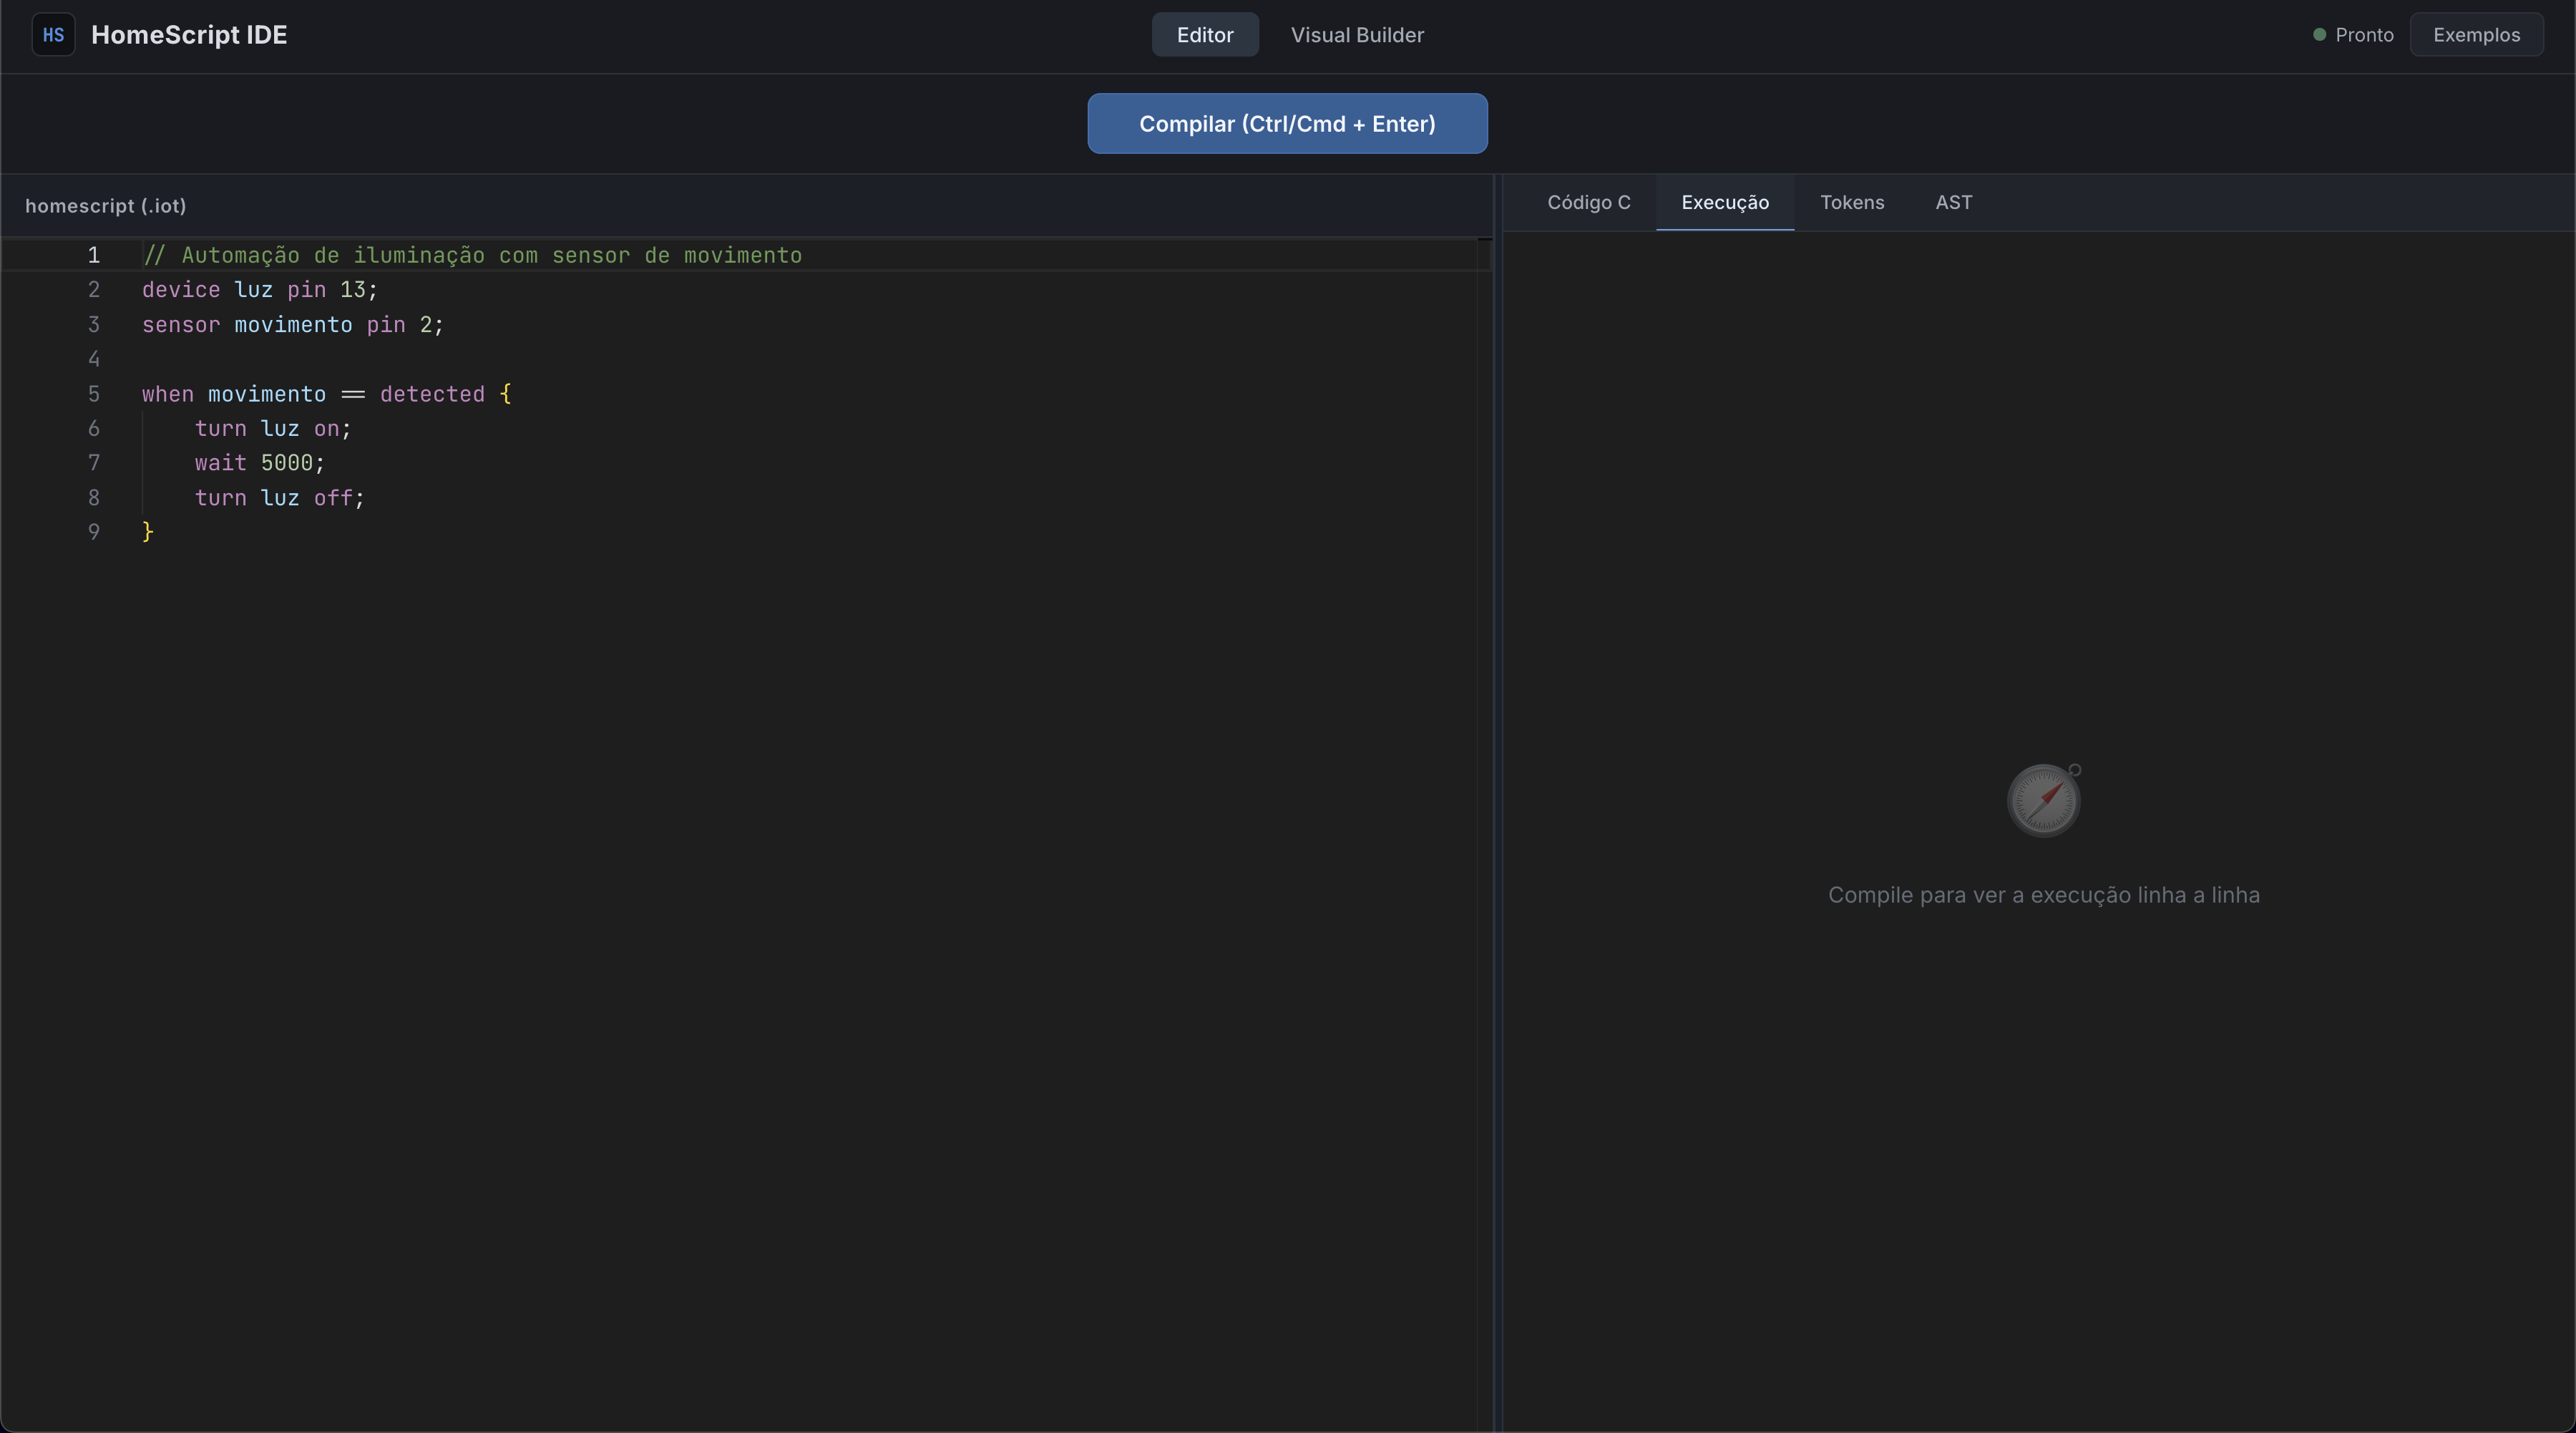
\includegraphics[width=0.95\linewidth]{../img/tela1.png}}
\caption{IDE HomeScript: editor Monaco à esquerda, painel de resultados à direita com abas Código C, Execução, Tokens e AST.}
\label{fig:ide}
\end{figure}

\subsection{Backend REST e IDE Web}

O backend (\texttt{backend/app.py}) usa FastAPI~\cite{fastapi2024} com
endpoints \texttt{POST /compile}, \texttt{POST /tokens}, \texttt{GET /health}
e \texttt{GET /exemplos}. A ponte (\texttt{compiler\_bridge.py}) cria um
arquivo temporário \texttt{.iot}, executa \texttt{homescript --json},
captura \texttt{stdout} e interpreta o JSON, com tratamento de
\texttt{FileNotFoundError}, \texttt{TimeoutExpired} e
\texttt{json.JSONDecodeError}.

O frontend usa Monaco Editor~\cite{monaco2024} configurado com linguagem
customizada \texttt{homescript}: tokenização com destaque para palavras-chave
EN e PT-BR, fechamento automático de blocos, mais de 30 entradas de
autocomplete com snippets para DHT11, HC-SR04, \texttt{if}/\texttt{when}/\texttt{for}/\texttt{while}
e equivalentes PT-BR. O painel de resultados possui quatro abas:
\textbf{Código C} (com cópia), \textbf{Tokens}, \textbf{AST} e
\textbf{Execução} (rastro passo a passo com função interna do lexer, snippet
de código C e caracteres consumidos por token). O Visual Builder
(Fig.~\ref{fig:visual}) permite montar automações graficamente e gera código
HomeScript válido ao confirmar.

\begin{figure}[htbp]
\centerline{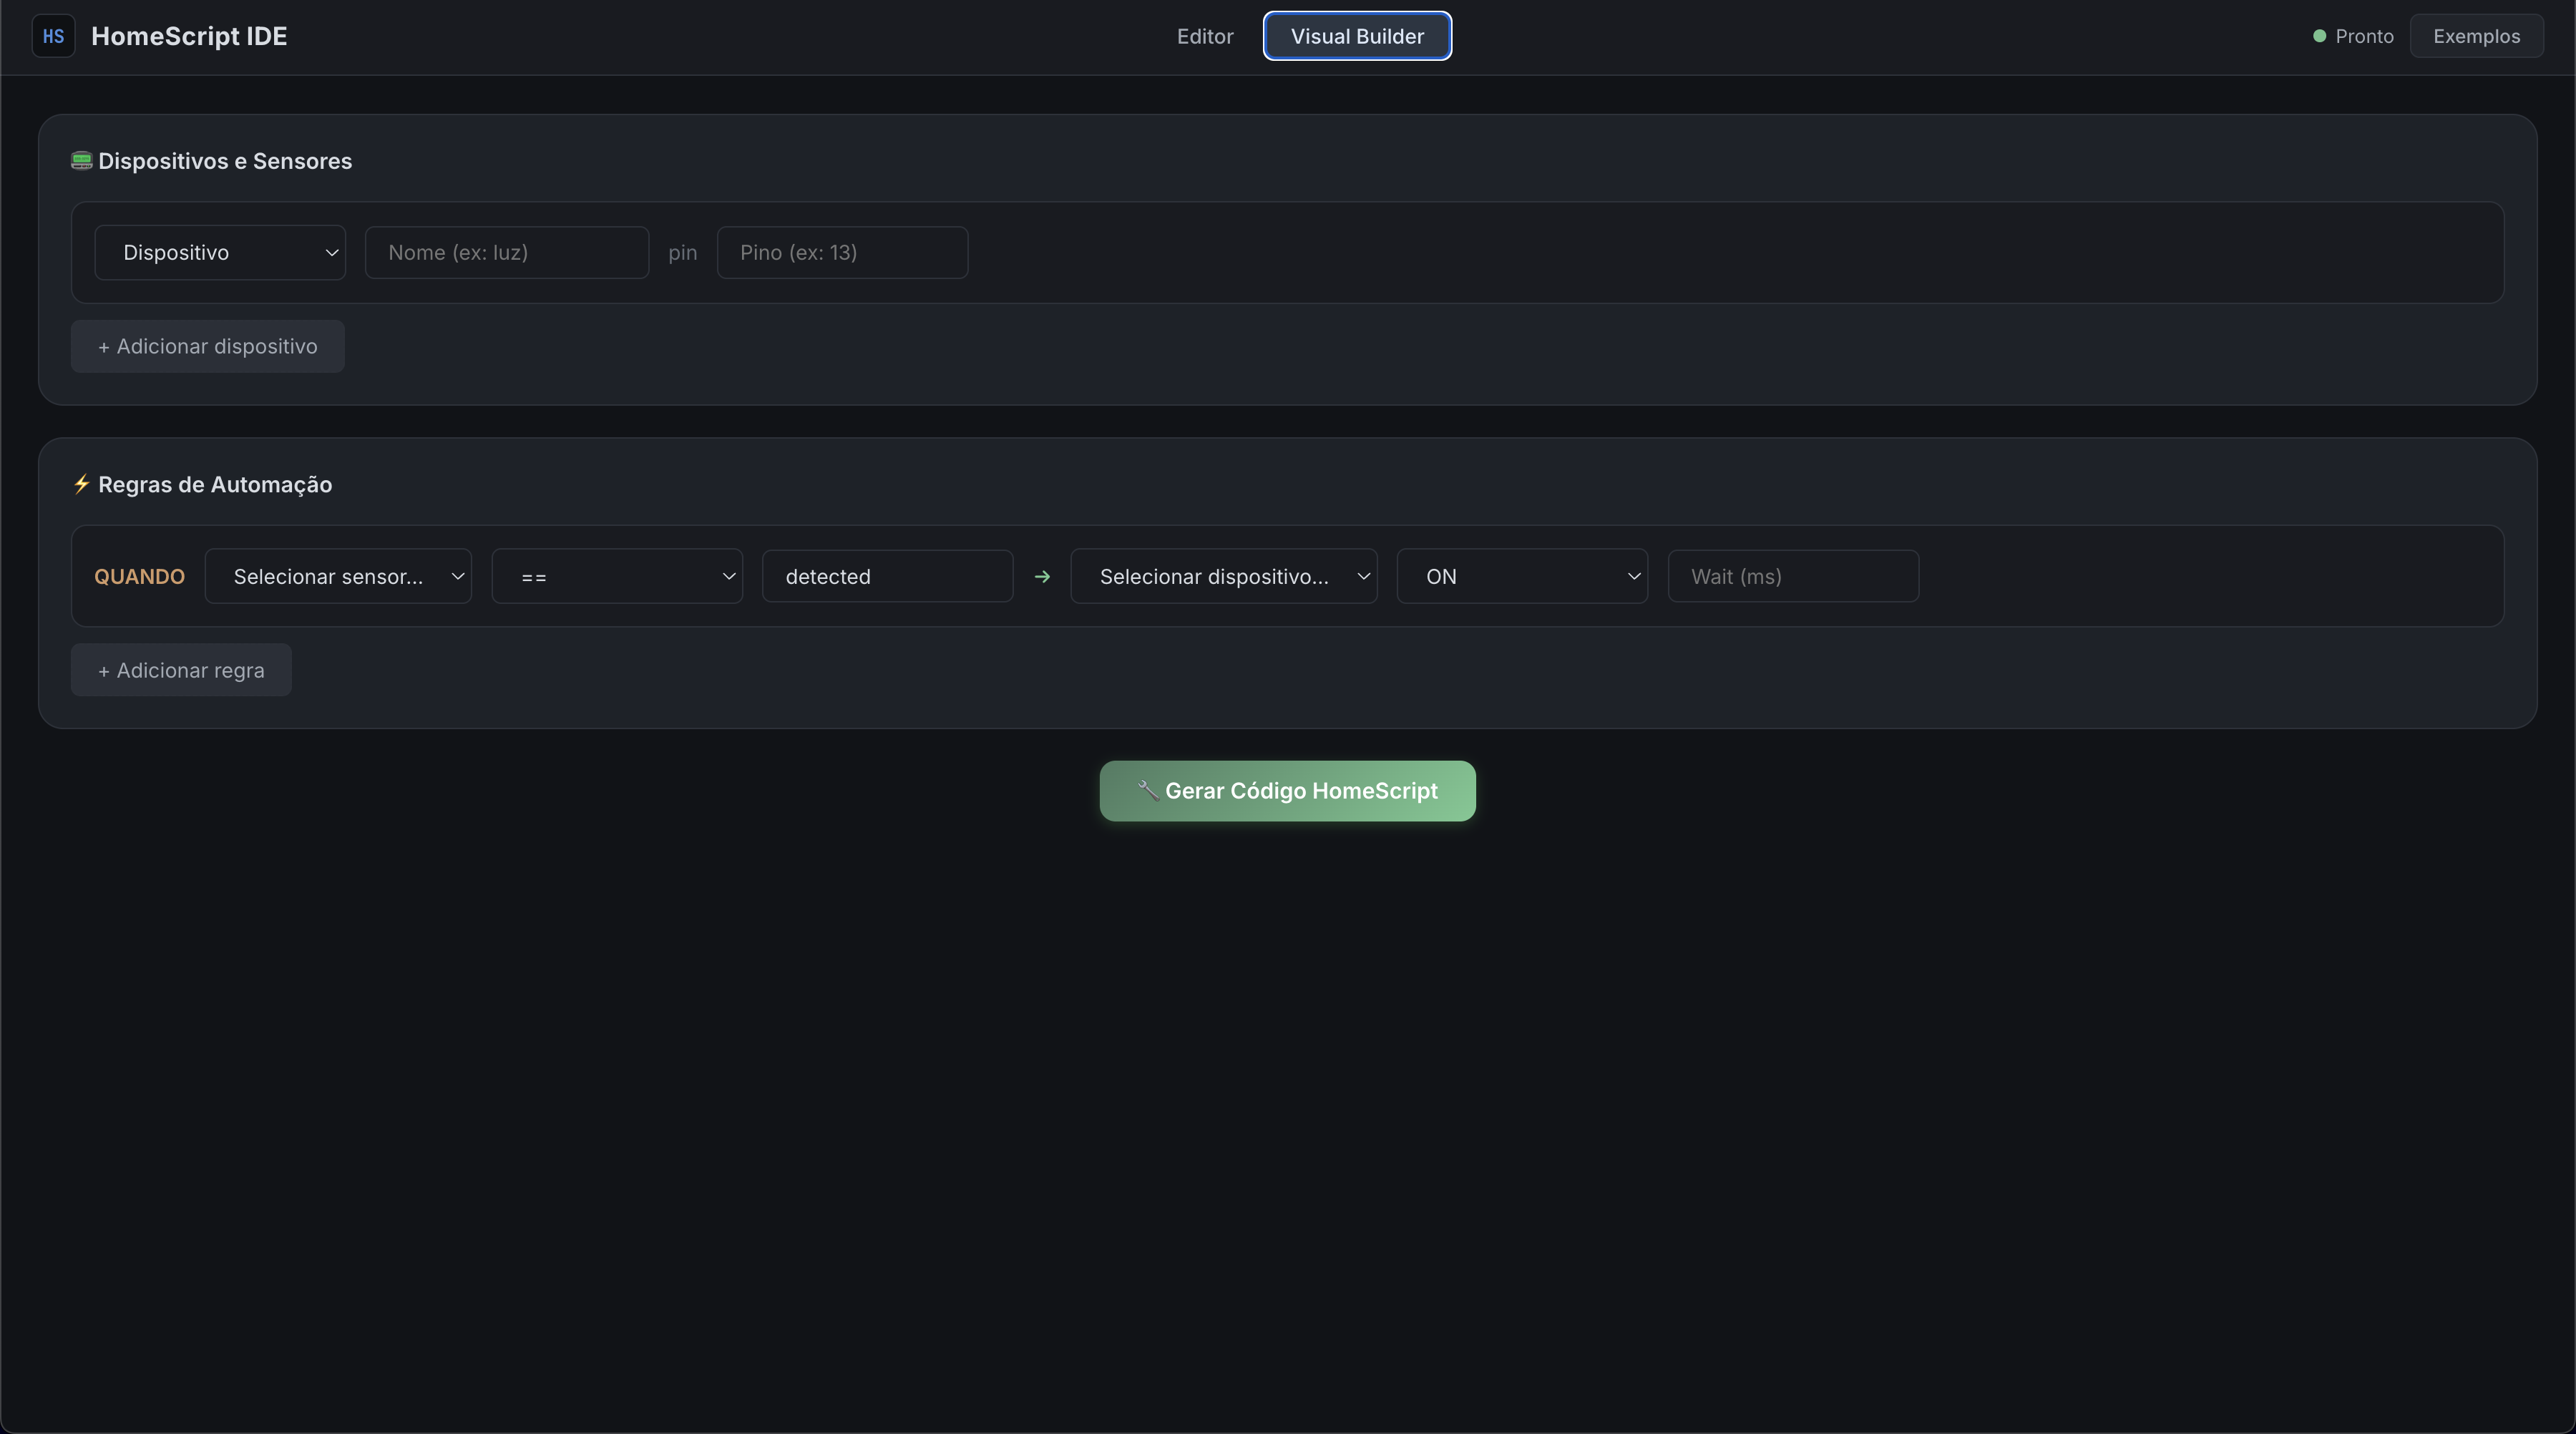
\includegraphics[width=0.95\linewidth]{../img/tela2.png}}
\caption{Visual Builder: interface gráfica para montagem de automações sem escrever código.}
\label{fig:visual}
\end{figure}

\subsection{Cenário de Validação: \texttt{casa\_completa\_plus.iot}}

Para a validação do pipeline completo foi utilizado o cenário
\texttt{casa\_completa\_plus.iot}, o mais abrangente do repositório. Ele
combina todos os recursos da linguagem em um único programa: dispositivos,
sensores de três tipos distintos (digital, analógico, DHT11 e HC-SR04),
variáveis, expressões aritméticas, condicionais com \texttt{senao} aninhado,
laços \texttt{para} e \texttt{enquanto}, e comandos de telemetria — tudo
escrito em PT-BR. A listagem~\ref{lst:cenario} apresenta o programa completo.

\begin{lstlisting}[style=homescript,caption={Cenário residencial completo em HomeScript (PT-BR).},label={lst:cenario}]
// Dispositivos (9 atuadores)
dispositivo luz_sala pino 13;
dispositivo luz_corredor pino 12;
dispositivo luz_jardim pino 11;
dispositivo ventilador_quarto pino 10;
dispositivo aquecedor_quarto pino 9;
dispositivo sirene pino 8;
dispositivo bomba_caixa pino 7;
dispositivo portao_motor pino 6;
dispositivo fita_led_garagem pino 5;

// Sensores (4 tipos)
sensor movimento_sala pino 2;
sensor porta_entrada pino 3;
sensor luminosidade_jardim pino A0;
sensor nivel_caixa pino A1;
sensor temperatura_quarto tipo dht11 pino 4;
sensor distancia_garagem tipo hcsr04 gatilho 14 eco 15;

// Variaveis de controle
let limite_luz_jardim = 450;
let temperatura_max = 29;
let temperatura_min = 23;
let nivel_minimo_caixa = 380;
let distancia_abertura_portao = 35;
let contador_alertas = 0;
let contador_movimento = 0;
let i = 0;
let tentativas_portao = 0;

// Rotina 1: presenca na sala (sensor digital)
quando movimento_sala == detectado {
    contador_movimento = contador_movimento + 1;
    ligar luz_sala;
    esperar 3000;
} senao {
    desligar luz_sala;
}

// Rotina 2: seguranca da porta com pulso (FOR)
quando porta_entrada == detectado {
    contador_alertas = contador_alertas + 1;
    ligar luz_corredor;
    para i = 0; i < 3; i = i + 1 {
        ligar sirene;
        esperar 250;
        desligar sirene;
        esperar 250;
    }
} senao {
    desligar luz_corredor;
}

// Rotina 3: iluminacao automatica (sensor analogico)
se luminosidade_jardim < limite_luz_jardim {
    ligar luz_jardim;
} senao {
    desligar luz_jardim;
}

// Rotina 4: conforto termico com DHT11 (if aninhado)
se temperatura_quarto > temperatura_max {
    ligar ventilador_quarto;
    desligar aquecedor_quarto;
} senao {
    se temperatura_quarto < temperatura_min {
        ligar aquecedor_quarto;
        desligar ventilador_quarto;
    } senao {
        desligar ventilador_quarto;
        desligar aquecedor_quarto;
    }
}

// Rotina 5: bomba d'agua (sintaxe EN/PT misturada)
if nivel_caixa < nivel_minimo_caixa {
    turn bomba_caixa on;
} else {
    turn bomba_caixa off;
}

// Rotina 6: portao inteligente com HC-SR04 (WHILE)
quando distancia_garagem < distancia_abertura_portao {
    tentativas_portao = 0;
    enquanto tentativas_portao < 2 {
        ligar portao_motor;
        ligar fita_led_garagem;
        esperar 1200;
        desligar portao_motor;
        esperar 300;
        tentativas_portao = tentativas_portao + 1;
    }
} senao {
    desligar portao_motor;
    desligar fita_led_garagem;
}

// Telemetria serial
print contador_movimento;
print contador_alertas;
print temperatura_max;
print distancia_abertura_portao;
\end{lstlisting}

A Tabela~\ref{tab:rotinas} resume as seis rotinas de automação e os recursos
de linguagem exercitados por cada uma.

\begin{table}[htbp]
\caption{Rotinas do cenário de validação e recursos exercitados}
\label{tab:rotinas}
\centering
\begin{tabular}{clp{0.45\linewidth}}
\toprule
\textbf{Rotina} & \textbf{Sensor/Recurso} & \textbf{Recursos exercitados} \\
\midrule
1 & PIR digital & \texttt{quando/senao}, \texttt{digitalRead}, variável, \texttt{esperar} \\
2 & Reed switch & \texttt{quando/senao}, laço \texttt{para}, 3 pulsos de buzzer \\
3 & LDR analógico & \texttt{se/senao}, \texttt{analogRead}, limiar por variável \\
4 & DHT11 & \texttt{se/senao} aninhado, cache de leitura, \texttt{isnan()} \\
5 & Potenciômetro & Sintaxe EN/PT misturada no mesmo arquivo \\
6 & HC-SR04 & \texttt{quando/senao}, \texttt{enquanto}, função auxiliar \\
\bottomrule
\end{tabular}
\end{table}

\subsection{Código C Gerado: Análise por Rotina}
\label{subsec:codegen_analise}

O compilador transforma o programa da listagem~\ref{lst:cenario} em código
C/Arduino completo, sem intervenção manual. A listagem~\ref{lst:preambulo}
apresenta o preâmbulo gerado.

\begin{lstlisting}[style=csmall,caption={Preâmbulo e declarações globais gerados.},label={lst:preambulo}]
#include <Arduino.h>
#include <math.h>
#include <DHT.h>

// Dispositivos como macros de pre-processador
#define luz_sala 13
#define luz_corredor 12
#define luz_jardim 11
#define ventilador_quarto 10
#define aquecedor_quarto 9
#define sirene 8
#define bomba_caixa 7
#define portao_motor 6
#define fita_led_garagem 5

// Variaveis de pino para sensores
int movimento_sala_pin = 2;
int porta_entrada_pin = 3;
int luminosidade_jardim_pin = A0;
int nivel_caixa_pin = A1;
DHT temperatura_quarto_dht(4, DHT11);
int distancia_garagem_trig_pin = 14;
int distancia_garagem_echo_pin = 15;

// Variaveis de controle (let -> int global)
int limite_luz_jardim = 450;
int temperatura_max = 29;
int temperatura_min = 23;
int nivel_minimo_caixa = 380;
int distancia_abertura_portao = 35;
int contador_alertas = 0;
int contador_movimento = 0;
int i = 0;
int tentativas_portao = 0;
\end{lstlisting}

Para o sensor HC-SR04, o codegen gera a função auxiliar de medição
(listagem~\ref{lst:hcsr04_fn}). O timeout de 30 ms no \texttt{pulseIn}
evita travamento da MCU na ausência de eco. A conversão
\texttt{duration / 58} é a aproximação inteira de
$d = \frac{t \cdot 343}{2 \times 10^{4}}$ cm.

\begin{lstlisting}[style=csmall,caption={Função auxiliar gerada para o HC-SR04.},label={lst:hcsr04_fn}]
long read_distancia_garagem_cm() {
    digitalWrite(distancia_garagem_trig_pin, LOW);
    delayMicroseconds(2);
    digitalWrite(distancia_garagem_trig_pin, HIGH);
    delayMicroseconds(10);
    digitalWrite(distancia_garagem_trig_pin, LOW);
    long duration = pulseIn(distancia_garagem_echo_pin,
                            HIGH, 30000);
    return duration / 58;
}
\end{lstlisting}

A função \texttt{setup()} gerada configura todos os pinos e inicializa os
sensores (listagem~\ref{lst:setup_gen}).

\begin{lstlisting}[style=csmall,caption={Função \texttt{setup()} gerada.},label={lst:setup_gen}]
void setup() {
    pinMode(luz_sala, OUTPUT);
    pinMode(luz_corredor, OUTPUT);
    pinMode(luz_jardim, OUTPUT);
    pinMode(ventilador_quarto, OUTPUT);
    pinMode(aquecedor_quarto, OUTPUT);
    pinMode(sirene, OUTPUT);
    pinMode(bomba_caixa, OUTPUT);
    pinMode(portao_motor, OUTPUT);
    pinMode(fita_led_garagem, OUTPUT);
    temperatura_quarto_dht.begin();
    pinMode(distancia_garagem_trig_pin, OUTPUT);
    pinMode(distancia_garagem_echo_pin, INPUT);
    digitalWrite(distancia_garagem_trig_pin, LOW);
    pinMode(movimento_sala_pin, INPUT);
    pinMode(porta_entrada_pin, INPUT);
    pinMode(luminosidade_jardim_pin, INPUT);
    pinMode(nivel_caixa_pin, INPUT);
    Serial.begin(9600);
}
\end{lstlisting}

No \texttt{loop()}, cada rotina HomeScript gera o código C correspondente.
As rotinas 1 e 2 (sensores digitais) são as mais diretas
(listagem~\ref{lst:rot12}).

\begin{lstlisting}[style=csmall,caption={Rotinas 1 e 2 geradas no \texttt{loop()}.},label={lst:rot12}]
// Rotina 1 - presenca na sala
if (digitalRead(movimento_sala_pin) == HIGH) {
    contador_movimento = contador_movimento + 1;
    digitalWrite(luz_sala, HIGH);
    delay(3000);
} else {
    digitalWrite(luz_sala, LOW);
}

// Rotina 2 - seguranca da porta com FOR
if (digitalRead(porta_entrada_pin) == HIGH) {
    contador_alertas = contador_alertas + 1;
    digitalWrite(luz_corredor, HIGH);
    for (i = 0; ; i = i + 1) {
        if (!(i < 3)) break;
        digitalWrite(sirene, HIGH);
        delay(250);
        digitalWrite(sirene, LOW);
        delay(250);
    }
} else {
    digitalWrite(luz_corredor, LOW);
}
\end{lstlisting}

A rotina 3 usa \texttt{analogRead} porque o pino é analógico (A0). O
gerador detecta o tipo do sensor e escolhe automaticamente a função de
leitura correta. A rotina 4 demonstra o mecanismo de cache de leituras DHT11
(listagem~\ref{lst:rot34}).

\begin{lstlisting}[style=csmall,caption={Rotinas 3 e 4 — analógico e DHT11 com cache.},label={lst:rot34}]
// Rotina 3 - sensor analogico (LDR em A0)
int leitura_luminosidade_jardim =
    analogRead(luminosidade_jardim_pin);
if (leitura_luminosidade_jardim < limite_luz_jardim) {
    digitalWrite(luz_jardim, HIGH);
} else {
    digitalWrite(luz_jardim, LOW);
}

// Rotina 4 - DHT11 com if/else aninhado
// Cache: uma unica leitura para ambos os ramos
float leitura_temperatura_quarto =
    temperatura_quarto_dht.readTemperature();
if (!isnan(leitura_temperatura_quarto) &&
    leitura_temperatura_quarto > temperatura_max) {
    digitalWrite(ventilador_quarto, HIGH);
    digitalWrite(aquecedor_quarto, LOW);
} else {
    // Ramo else reutiliza leitura_temperatura_quarto
    if (!isnan(leitura_temperatura_quarto) &&
        leitura_temperatura_quarto < temperatura_min) {
        digitalWrite(aquecedor_quarto, HIGH);
        digitalWrite(ventilador_quarto, LOW);
    } else {
        digitalWrite(ventilador_quarto, LOW);
        digitalWrite(aquecedor_quarto, LOW);
    }
}
\end{lstlisting}

A rotina 4 evidencia três características relevantes do gerador: (1) detecção
automática do tipo de sensor DHT11 via \texttt{sensor\_tipo} da AST; (2)
inserção da guarda \texttt{!isnan()} para proteger contra leituras inválidas
do sensor; (3) materialização de uma única variável temporária
\texttt{leitura\_temperatura\_quarto} reutilizada em ambos os ramos do
\texttt{if}/\texttt{else} aninhado — evitando duas chamadas a
\texttt{readTemperature()} (cada uma demora $\sim$250 ms).

As rotinas 5 e 6 demonstram respectivamente a interoperabilidade EN/PT-BR
no mesmo arquivo e o laço \texttt{while} com HC-SR04
(listagem~\ref{lst:rot56}).

\begin{lstlisting}[style=csmall,caption={Rotinas 5 e 6 — bomba e portão com WHILE.},label={lst:rot56}]
// Rotina 5 - bomba dagua (sintaxe EN no meio do PT-BR)
int leitura_nivel_caixa =
    analogRead(nivel_caixa_pin);
if (leitura_nivel_caixa < nivel_minimo_caixa) {
    digitalWrite(bomba_caixa, HIGH);
} else {
    digitalWrite(bomba_caixa, LOW);
}

// Rotina 6 - portao com HC-SR04 e WHILE
long leitura_distancia_garagem =
    read_distancia_garagem_cm();
if (leitura_distancia_garagem < distancia_abertura_portao) {
    tentativas_portao = 0;
    while (1) {
        if (!(tentativas_portao < 2)) break;
        digitalWrite(portao_motor, HIGH);
        digitalWrite(fita_led_garagem, HIGH);
        delay(1200);
        digitalWrite(portao_motor, LOW);
        delay(300);
        tentativas_portao = tentativas_portao + 1;
    }
} else {
    digitalWrite(portao_motor, LOW);
    digitalWrite(fita_led_garagem, LOW);
}

// Telemetria serial
Serial.println(contador_movimento);
Serial.println(contador_alertas);
Serial.println(temperatura_max);
Serial.println(distancia_abertura_portao);
\end{lstlisting}

A rotina 6 evidencia a composição de laços: o \texttt{enquanto} interno
aciona o motor por dois pulsos de 1 200 ms cada, com pausa de 300 ms entre
eles. O padrão \texttt{while(1) \{ if(!(cond)) break; \}} garante que a
condição (\texttt{tentativas\_portao < 2}) seja reavaliada a cada iteração.

\subsection{Protótipo Físico: Montagem e Validação}

O código C produzido pela listagem~\ref{lst:preambulo}--\ref{lst:rot56}
foi carregado diretamente em um Arduino Uno (ATMega328P) via IDE Arduino
sem qualquer modificação manual. A Tabela~\ref{tab:hardware_pins} descreve
o mapeamento completo de pinos e componentes do protótipo.

\begin{table}[htbp]
\caption{Mapeamento de pinos e periféricos do protótipo físico}
\label{tab:hardware_pins}
\centering
\begin{tabular}{p{0.33\linewidth}lc}
\toprule
\textbf{Identificador no código} & \textbf{Componente} & \textbf{Pino} \\
\midrule
\texttt{luz\_sala}          & LED / Relé         & 13 \\
\texttt{luz\_corredor}      & LED                & 12 \\
\texttt{luz\_jardim}        & LED                & 11 \\
\texttt{ventilador\_quarto} & Motor DC           & 10 \\
\texttt{aquecedor\_quarto}  & Resistor aquecedor &  9 \\
\texttt{sirene}             & Buzzer piezoelétrico & 8 \\
\texttt{bomba\_caixa}       & Microbomba DC      &  7 \\
\texttt{portao\_motor}      & Servomotor         &  6 \\
\texttt{fita\_led\_garagem} & Fita de LEDs       &  5 \\
\texttt{movimento\_sala}    & Sensor PIR         &  2 \\
\texttt{porta\_entrada}     & Reed switch        &  3 \\
\texttt{temperatura\_quarto}& DHT11              &  4 \\
\texttt{luminosidade\_jardim}& LDR + resistor    & A0 \\
\texttt{nivel\_caixa}       & Potenciômetro      & A1 \\
\texttt{distancia\_garagem} & HC-SR04 (trig/echo)& 14/15 \\
\bottomrule
\end{tabular}
\end{table}

\begin{figure}[htbp]
\centerline{%
\fbox{\parbox{0.9\linewidth}{\centering\vspace{1.8cm}
\textit{[Inserir foto do protótipo físico montado]}\\
Arduino Uno + 9 atuadores + 6 sensores\\
\vspace{1.8cm}}}}
\caption{Protótipo físico: Arduino Uno com 9 atuadores e 6 sensores validando o código gerado pelo compilador HomeScript.}
\label{fig:arduino}
\end{figure}

Os parâmetros operacionais utilizados na validação são apresentados na
Tabela~\ref{tab:limiares}.

\begin{table}[htbp]
\caption{Parâmetros operacionais usados na validação física}
\label{tab:limiares}
\centering
\begin{tabular}{p{0.44\linewidth}cc}
\toprule
\textbf{Variável HomeScript} & \textbf{Valor} & \textbf{Unidade} \\
\midrule
\texttt{limite\_luz\_jardim}         & 450 & ADC (0--1023) \\
\texttt{temperatura\_max}            &  29 & $^{\circ}$C \\
\texttt{temperatura\_min}            &  23 & $^{\circ}$C \\
\texttt{nivel\_minimo\_caixa}        & 380 & ADC \\
\texttt{distancia\_abertura\_portao} &  35 & cm \\
\bottomrule
\end{tabular}
\end{table}

Três aspectos do código gerado foram verificados experimentalmente:

\textbf{(1) Protocolo HC-SR04 (Rotina 6).} A função
\texttt{read\_distancia\_garagem\_cm()} executou corretamente a sequência:
\texttt{trig} LOW por 2 $\mu$s, HIGH por 10 $\mu$s, LOW; leitura do eco
via \texttt{pulseIn} com timeout de 30 ms; conversão para centímetros.
Os pinos 14 e 15 foram utilizados como I/O digital (mapeados como A0/A1 no
Uno), dado o esgotamento dos pinos digitais convencionais. Ao aproximar a
mão a menos de 35 cm do sensor, o \texttt{portao\_motor} ativou dois pulsos
de 1 200 ms com intervalo de 300 ms, reproduzindo exatamente o laço
\texttt{enquanto} da Rotina 6.

\textbf{(2) Laço \texttt{para} com buzzer (Rotina 2).} Ao fechar o reed
switch simulando abertura da porta, o buzzer emitiu exatamente 3 pulsos de
250 ms (ligado/desligado), totalizando 1 500 ms de sinalização. O laço
\texttt{for} gerado iterou corretamente de \texttt{i = 0} até
\texttt{i < 3}, confirmando a inicialização, condição e incremento.

\textbf{(3) Controle térmico com DHT11 e cache (Rotina 4).} O bloco
condicional aninhado impediu a ativação simultânea do ventilador e do
aquecedor. Com temperatura entre 23 °C e 29 °C, ambos permaneceram em
\texttt{LOW}. Acima de 29 °C, apenas o ventilador ativou; abaixo de
23 °C, apenas o aquecedor. O cache de leitura garantiu que apenas uma
chamada a \texttt{readTemperature()} foi feita por ciclo do \texttt{loop()},
evitando o atraso de 500 ms que ocorreria com duas leituras independentes.

Os dados de telemetria enviados via \texttt{Serial.println()} a 9 600 bauds
confirmaram os valores das variáveis \texttt{contador\_movimento},
\texttt{contador\_alertas}, \texttt{temperatura\_max} e
\texttt{distancia\_abertura\_portao} a cada ciclo, validando a corretude
semântica do código gerado de ponta a ponta: da linguagem HomeScript ao
comportamento físico observável.

% -------------------------------------------------------
\section{Conclusão e Trabalhos Futuros}
\label{sec:conclusao}

O projeto HomeScript demonstrou que é possível implementar um compilador
completo como sistema acadêmico funcional com proposta de produto real. A
linguagem cobre um domínio bem definido com sintaxe acessível; o compilador
produz código C correto para múltiplos tipos de sensor sem intervenção do
usuário; e a IDE web torna o pipeline de compilação observável e pedagógico.
A validação física com o cenário \texttt{casa\_completa\_plus.iot} confirmou
a corretude do pipeline de ponta a ponta — do arquivo \texttt{.iot} ao
comportamento de 15 componentes de hardware.

As principais contribuições técnicas são: \textbf{(1)} lexer manual com
bilinguismo EN/PT-BR no nível de tokens; \textbf{(2)} parser recursivo
descendente com expressões aritméticas e precedência de operadores codificada
na hierarquia de chamadas; \textbf{(3)} análise semântica com validação de
tipos de sensor, conflitos de pino e escopo de variáveis;
\textbf{(4)} gerador de código com cache de leituras de sensor para blocos
\texttt{if}/\texttt{else} sobre o mesmo sensor; e \textbf{(5)} IDE web com
rastro passo a passo do pipeline e construtor visual de automações.

O principal aprendizado é que a qualidade de um compilador depende tanto da
teoria das fases~\cite{aho2006} quanto da engenharia de erros: mensagens
localizadas com linha e coluna, formatos intermediários bem definidos (JSON)
e integração consistente entre fases são fatores tão importantes quanto a
corretude do algoritmo de análise.

Como trabalhos futuros: suporte a ponto flutuante e cadeias de caracteres;
AST própria para expressões aritméticas; geração para ESP32 com Wi-Fi e
MQTT~\cite{mqtt2019}; simulador de execução integrado; exportação direta
de arquivo \texttt{.ino}; e isolamento de processos no backend.

\section*{Agradecimentos}
A equipe agradece ao professor da disciplina de Linguagens Formais e
Compiladores pela orientação e pela exigência do modelo IEEE.

\balance
\begin{thebibliography}{00}

\bibitem{aho2006}
A.~V. Aho, M.~S. Lam, R.~Sethi, e J.~D. Ullman,
\textit{Compilers: Principles, Techniques, and Tools}, 2nd~ed.
Addison-Wesley, 2006.

\bibitem{cooper2011}
K.~D. Cooper e L.~Torczon,
\textit{Engineering a Compiler}, 2nd~ed.
Morgan Kaufmann, 2011.

\bibitem{mernik2005}
M.~Mernik, J.~Heering, e A.~M. Sloane,
``When and how to develop domain-specific languages,''
\textit{ACM Comput. Surv.}, vol.~37, no.~4, pp.~316--344, Dez. 2005.

\bibitem{fowler2010}
M.~Fowler,
\textit{Domain-Specific Languages}.
Addison-Wesley, 2010.

\bibitem{vandeursen2000}
A.~van Deursen, P.~Klint, e J.~Visser,
``Domain-specific languages: An annotated bibliography,''
\textit{ACM SIGPLAN Not.}, vol.~35, no.~6, pp.~26--36, Jun. 2000.

\bibitem{parr2013}
T.~Parr,
\textit{The Definitive ANTLR 4 Reference}.
Pragmatic Bookshelf, 2013.

\bibitem{wirth1976}
N.~Wirth,
\textit{Algorithms + Data Structures = Programs}.
Prentice Hall, 1976.

\bibitem{lattner2004}
C.~Lattner e V.~Adve,
``LLVM: A compilation framework for lifelong program analysis \& transformation,''
in \textit{Proc. CGO}, 2004, pp.~75--86.

\bibitem{atzori2010}
L.~Atzori, A.~Iera, e G.~Morabito,
``The Internet of Things: A survey,''
\textit{Comput. Netw.}, vol.~54, no.~15, pp.~2787--2805, Out. 2010.

\bibitem{alfuqaha2015}
A.~Al-Fuqaha, M.~Guizani, M.~Mohammadi, M.~Aledhari, e M.~Ayyash,
``Internet of Things: A survey on enabling technologies, protocols, and
applications,''
\textit{IEEE Commun. Surv. Tutorials}, vol.~17, no.~4, pp.~2347--2376, 2015.

\bibitem{zanella2014}
A.~Zanella, N.~Bui, A.~Castellani, L.~Vangelista, e M.~Zorzi,
``Internet of Things for smart cities,''
\textit{IEEE Internet Things J.}, vol.~1, no.~1, pp.~22--32, Fev. 2014.

\bibitem{banzi2011}
M.~Banzi,
\textit{Getting Started with Arduino}, 2nd~ed.
O'Reilly Media, 2011.

\bibitem{kr1988}
B.~W. Kernighan e D.~M. Ritchie,
\textit{The C Programming Language}, 2nd~ed.
Prentice Hall, 1988.

\bibitem{fastapi2024}
S.~Ramírez,
``FastAPI: Modern, fast web framework for building APIs with Python,''
2024. [Online]. Disponível: \url{https://fastapi.tiangolo.com/}

\bibitem{react2024}
Meta Platforms,
``React: A JavaScript library for building user interfaces,''
2024. [Online]. Disponível: \url{https://react.dev/}

\bibitem{monaco2024}
Microsoft,
``Monaco Editor,''
2024. [Online]. Disponível:
\url{https://microsoft.github.io/monaco-editor/}

\bibitem{arduino2024}
Arduino,
``Arduino Language Reference,''
2024. [Online]. Disponível: \url{https://www.arduino.cc/reference/en/}

\bibitem{mqtt2019}
OASIS Standard,
``MQTT Version 5.0,'' Mar. 2019. [Online]. Disponível:
\url{https://docs.oasis-open.org/mqtt/mqtt/v5.0/mqtt-v5.0.html}

\bibitem{docs-def}
Projeto HomeScript,
\textit{Definição da Linguagem HomeScript},
\texttt{docs/definicao\_linguagem.md}, 2026.

\bibitem{docs-tokens}
Projeto HomeScript,
\textit{Tabela de Tokens e Expressões Regulares},
\texttt{docs/tabela\_tokens.md} e \texttt{docs/regex.md}, 2026.

\end{thebibliography}

\end{document}
